\documentclass[11pt,twoside]{article}
\usepackage{geometry}
\usepackage{enumerate}
\usepackage{latexsym,booktabs}
\usepackage{amsmath,amssymb}
\usepackage{graphicx}
\usepackage[singlespacing]{setspace}

\geometry{a4paper,left=2cm,right=2.0cm, top=2cm, bottom=2.0cm}

\newtheorem{Definition}{Definition}
\newtheorem{Theorem}{Theorem}
\newtheorem{Lemma}{Lemma}
\newtheorem{Corollary}{Corollary}
\newtheorem{Proposition}{Proposition}
\newtheorem{Algorithm}{Algorithm}
\numberwithin{Theorem}{section}
\numberwithin{Definition}{section}
\numberwithin{Lemma}{section}
\numberwithin{Algorithm}{section}
\numberwithin{equation}{section}


% *********************************************************************
% Headings and page layout
% *********************************************************************
\usepackage{fancyhdr} % to design my own headings
\usepackage{titlesec, titletoc} % to design my own toc and part/chapter/section styles

% page style of "chapter"
\titleformat{\chapter}[display]{\LARGE \bfseries}
	{\Large Chapter \thesection \thispagestyle{plain}}{0ex}{\titlerule\vspace{2ex}}
\titlespacing*{\chapter}{0ex}{-8ex}{8ex}

\titleformat{\section}[display]{\LARGE \bfseries}
	{\Large Section \thesection \thispagestyle{plain}}{0ex}{\titlerule\vspace{2ex}}
\titlespacing*{\section}{0ex}{-8ex}{8ex}

% definition of headings
\fancypagestyle{memo}{
	\pagestyle{fancy}
	\fancyhf{}
	\fancyhead[RO,LE]{\thepage}
	\fancyhead[RE]{\rightmark}
	\fancyhead[LO]{\leftmark}
	\renewcommand\headrulewidth{0.5pt}
}



\begin{document}

\pagestyle{empty}

% =============================================================================
% Title page
% =============================================================================
\begin{titlepage}
\vspace*{.5em}
\center
\textbf{\large{The School of Mathematics}} \\
\vspace*{1em}
\begin{figure}[!h]
\centering

\includegraphics[width=180pt]{CentredLogoCMYK.jpg}
\end{figure}
\vspace{2em}
\textbf{\Huge{My Incredible Thesis}}\\[2em]
\textbf{\LARGE{by}}\\
\vspace{2em}
\textbf{\LARGE{My Name}}\\
\vspace{6.5em}
\Large{Dissertation Presented for the Degree of\\
MSc in Operational Research (with ...)}\\
\vspace{6.5em}
\Large{August 2019}\\
\vspace{3em}
\Large{Supervised by\\Dr Very Important}
\vfill
\end{titlepage}

\cleardoublepage


% =============================================================================
% Abstract, acknowledgments, and own work declaration
% =============================================================================
\begin{center}
\Large{Abstract}
\end{center}

Here comes your abstract ...

\clearpage

\begin{center}
\Large{Acknowledgments}
\end{center}

Here come your acknowledgments ...

\clearpage

\begin{center}
\Large{Own Work Declaration}
\end{center}

Here comes your own work declaration

\cleardoublepage



% =============================================================================
% Table of contents, tables, and pictures (if applicable)
% =============================================================================
\pagestyle{memo}

\setcounter{page}{1}
\pagenumbering{Roman}

% Table of contents
\thispagestyle{plain}
\tableofcontents
\clearpage

% Table of tables (if applicable)
\thispagestyle{plain}
\listoftables
\clearpage

% Table of pictures (if applicable)
\thispagestyle{plain}
\listoffigures
\cleardoublepage

\pagenumbering{arabic}
\setcounter{page}{1}

\nocite{*}
\bibliographystyle{abbrv}
\cleardoublepage % always start a new section on an odd page

\section{Introduction}
\label{sec.intro}

Here I will write a very good, precise and brief introduction.
Particularly Section \ref{sec:background} is good!
\cleardoublepage % always start a new section on an odd page


\section{Background}
\label{sec:background}

In the following, I explain some background stuff. I should really cut this short, but BlaBlaBlaBla BlaBlaBlaBlaBla Bla Bla BlaBlaBla Bla Bla BlaBlaBla Bla BlaBla BlaBla Bla BlaBlaBlaBla Bla BlaBla Bla Bla Bla BlaBla BlaBlaBlaBla BlaBlaBlaBlaBla Bla Bla BlaBlaBla Bla. Bla BlaBlaBla Bla BlaBla BlaBla Bla BlaBlaBlaBla Bla BlaBla Bla Bla Bla BlaBla BlaBlaBlaBla. BlaBlaBlaBlaBla Bla Bla BlaBlaBla Bla Bla BlaBlaBla Bla BlaBla BlaBla Bla BlaBlaBlaBla Bla BlaBla Bla Bla Bla BlaBla BlaBlaBlaBla BlaBlaBlaBlaBla Bla Bla BlaBlaBla Bla Bla BlaBlaBla Bla BlaBla BlaBla Bla BlaBlaBlaBla Bla BlaBla Bla Bla Bla BlaBla BlaBlaBlaBla BlaBlaBlaBlaBla Bla Bla BlaBlaBla Bla Bla BlaBlaBla Bla BlaBla BlaBla Bla. BlaBlaBlaBla Bla BlaBla Bla Bla Bla BlaBla BlaBlaBlaBla BlaBlaBlaBlaBla Bla Bla BlaBlaBla Bla Bla BlaBlaBla Bla BlaBla BlaBla Bla BlaBlaBlaBla Bla BlaBla Bla Bla Bla BlaBla.

Note that I start a new paragraph when I have an empty line like this. BlaBlaBlaBla BlaBlaBlaBlaBla Bla Bla BlaBlaBla Bla Bla BlaBlaBla Bla BlaBla BlaBla Bla BlaBlaBlaBla Bla BlaBla Bla Bla Bla. BlaBla BlaBlaBlaBla BlaBlaBlaBlaBla Bla Bla BlaBlaBla Bla Bla BlaBlaBla Bla BlaBla BlaBla Bla BlaBlaBlaBla Bla BlaBla Bla Bla Bla BlaBla BlaBlaBlaBla BlaBlaBlaBlaBla Bla Bla BlaBlaBla Bla Bla BlaBlaBla. Bla BlaBla BlaBla Bla BlaBlaBlaBla Bla BlaBla Bla Bla Bla BlaBla BlaBlaBlaBla BlaBlaBlaBlaBla Bla Bla BlaBlaBla Bla Bla BlaBlaBla Bla. BlaBla BlaBla Bla BlaBlaBlaBla Bla BlaBla Bla Bla Bla BlaBla BlaBlaBlaBla BlaBlaBlaBlaBla Bla Bla BlaBlaBla Bla Bla BlaBlaBla Bla BlaBla BlaBla Bla BlaBlaBlaBla Bla BlaBla Bla Bla Bla BlaBla.\\
But I can also end a line with a double backslash.
\clearpage

\subsection{Models}
\label{sec:Models}

Models are \emph{very} helpful because.
\begin{itemize}
 \item They're good.
 \item They're helpful.
\end{itemize}
\clearpage

\subsection{Techniques}
\label{sec:Techniques}

Techniques even better because.
\begin{enumerate}
 \item They're magnificent.
 \item If they work.
\end{enumerate}
\cleardoublepage % always start a new section on an odd page


\section{Technical Stuff}

Now it's getting very technical \ldots{} I will cite \cite{shiina,groewe2001}. I will also show my incredible $\alpha$, $\beta$ and $\gamma$ mathematics and do some other fancy stuff.

\subsection{Formulae}

For example look at this
\begin{equation}\label{eqn:aProblem}
\min{}\sum_{s\in\mathcal{S}}Pr_{s}\left[\sum_{t=1}^{T}\left(
\sum_{g\in\mathcal{G}}\left(\alpha_{gts}C_{g}^{0}+
p_{gts}C_{g}^{1}+\left(p_{gts}\right)^{2}C_{g}^{2}\right)
+\sum_{g\in\mathcal{C}}\gamma_{gts}C_{g}^{s}\right)\right],
\end{equation}
and you will see that it has a little number on the side so that I can refer to it as equation (\ref{eqn:aProblem}). Now if I do this
\begin{eqnarray}
\sum_{i=1}^{n}k_{i}&=&20\label{eqn:one}\\
\sum_{j=20}^{m}\delta_{i}&\geq{}&\eta{}\notag
\end{eqnarray}
I can align two formulae and control which one has a number on the side. It is (\ref{eqn:one}). I can also do something like this
\begin{displaymath}
Y_{l}=\left[\begin{array}{cc}
             \left(y_{s}+i\frac{b_{c}}{2}\right)\frac{1}{\tau{}^{2}} &
             -y_{s}\frac{1}{\tau{}e^{-i\theta^{s}}}\\
             -y_{s}\frac{1}{\tau{}e^{i\theta^{s}}} &
             y_{s}+i\frac{b_{c}}{2}
             \end{array}\right],
\end{displaymath}
and it won't have a number on the side. Now if I have to do some huge mathematics I'd better structure it a little and include linebreaks etc. so that it fits on one page.
\begin{eqnarray}\label{eqn:horrible}
p_{l}^{f}&=&G_{l11}\left(2v_{F(l)}\bar{v}_{F(l)}-\bar{v}_{F(l)}^{2}\right)\\
&+&
\bar{v}_{F(l)}\bar{v}_{T(l)}
\left[
B_{l12}\sin{}(\bar{\delta{}}_{F(l)}-\bar{\delta{}}_{T(l)})
+G_{l12}\cos{}(\bar{\delta{}}_{F(l)}-\bar{\delta{}}_{T(l)})
\right]\notag\\
&+&
\left[\begin{array}{r}
      \bar{v}_{T(l)}
      \left[
      B_{l12}\sin{}(\bar{\delta{}}_{F(l)}-\bar{\delta{}}_{T(l)})
      +G_{l12}\cos{}(\bar{\delta{}}_{F(l)}-\bar{\delta{}}_{T(l)})
      \right]\\
      \bar{v}_{F(l)}
      \left[
      B_{l12}\sin{}(\bar{\delta{}}_{F(l)}-\bar{\delta{}}_{T(l)})
      +G_{l12}\cos{}(\bar{\delta{}}_{F(l)}-\bar{\delta{}}_{T(l)})
      \right]\\
      \bar{v}_{F(l)}\bar{v}_{T(l)}
      \left[
      B_{l12}\cos{}(\bar{\delta{}}_{F(l)}-\bar{\delta{}}_{T(l)})
      -G_{l12}\sin{}(\bar{\delta{}}_{F(l)}-\bar{\delta{}}_{T(l)})
      \right]\\
      \bar{v}_{F(l)}\bar{v}_{T(l)}
      \left[
      -B_{l12}\cos{}(\bar{\delta{}}_{F(l)}-\bar{\delta{}}_{T(l)})
      +G_{l12}\sin{}(\bar{\delta{}}_{F(l)}-\bar{\delta{}}_{T(l)})
      \right]\\
      \end{array}\right]
\cdot{}
\left[\begin{array}{c}
      v_{F(l)}-\bar{v}_{F(l)}\\
      v_{T(l)}-\bar{v}_{T(l)}\\
      \delta_{F(l)}-\bar{\delta{}}_{F(l)}\\
      \delta_{T(l)}-\bar{\delta{}}_{T(l)}
      \end{array}\right],\notag
\end{eqnarray}
This is a lot of fun!
\clearpage

\subsection{Important Things}
Finally we should have a nice picture like this one. However, I won't forget that figures and table are environments which float around in my document. So LaTeX will place them wherever it thinks they fit well with the surrounding text. I can try to change that with a float specifier, e.g. [!ht].
%This is a comment. The Compiler ignores it. It is here to remind me that, if I use a .jpeg or .png picture file as below I will need to compile the document with the pdflatex compiler.
\begin{figure}[!ht]
\centering
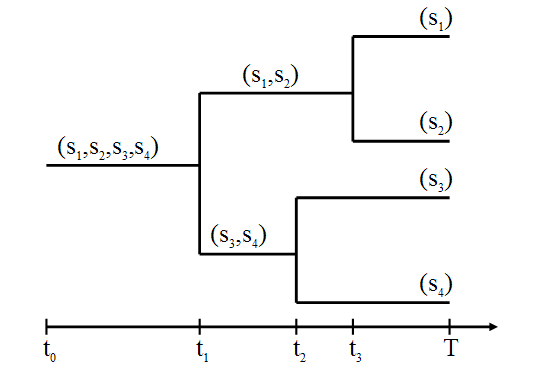
\includegraphics[width=0.5\textwidth]{scenTree.png}
\caption{Look at this scenario tree with funny times $t_{1}$ and scenarios $s_{1}$ etc.}
\label{fig:scenarioTree}
\end{figure}
Now I want to use one of my own environments. I want to define something.
\begin{Definition}
 I define
$$
\Gamma_{\eta}:=\sum_{i=1}^{n}\sum_{j=i}^{n}\xi{}(i,j)
$$
\end{Definition}
I definitely need some good tables, so I do this.
\begin{table}[!ht]
\centering
\begin{tabular}{|ll|rrrr|}
\hline
Case&Generators&Therm. Units&Lines&Peak load: [MW]&[MVar]\\
\hline\hline
6 bus&3 at 3 buses&2&11&210&210\\
9 bus&3 at 3 buses&3&9&315&115\\
24 bus&33 at 11 buses&26&38&2850&580\\
30 bus&6 at 6 buses&5&41&189.2&107.2\\
39 bus&10 at 10 buses&7&46&6254.2&1387.1\\
57 bus&7 at 7 buses&7&80&1250.8&336.4\\
\hline
\end{tabular}
\caption{Something that doesn't make sense.}
\label{tab:things}
\end{table}
I should really refer to Table \ref{tab:things}.

\subsection{And now something else}

\noindent
Let:
\begin{eqnarray*}
\Omega_0 & = & \{(x,y,z,f): \text{ satisfying } (9)-(19)\}, \\
\Omega_1 & = & \{(x,y,z,f): \text{ satisfying } (9),(11)-(20)\}, \\
\overline{\Omega}_0 & = & \{\textbf{0}\leq (x,y,z,f) \leq \textbf{1}: \text{ satisfying } (9)-(18)\}, \\
\overline{\Omega}_1 & = & \{\textbf{0}\leq (x,y,z,f) \leq \textbf{1}: \text{ satisfying } (9),(11)-(18),(20)\} \,.
\end{eqnarray*}
%
where $\textbf{0}$ and $\textbf{1}$ are vectors of appropriate dimensions with 0's and 1's, respectively.
Next we see that both $\Omega_0$ and $\Omega_1$ give equivalent formulations for the A-MSSP. In particular, the following statements hold:

\begin{Proposition}
$\Omega_0 \subseteq \Omega_1$.
\end{Proposition}

\noindent
\textbf{Proof.}
Let us suppose there exists $(x,y,z,f) \in \Omega_1$ such that $(x,y,z,f) \notin \Omega_0$.
Then, there exist indices $i \in I$ and $t \in \{0,\ldots,|T|-s_i\} $ with $x_i^t > \displaystyle 0.5\,\left( \sum_{h=1}^{s_i} x_i^{t+h} +1\right)$.
By definition, $x_i^t = 1$ and $x_i^{t+h} = 0$ for all $h \in \{1,\dots,s_i\}$. By~(11) and (12), $\displaystyle \sum_{h=1}^{s_i} f_i^{th}=1$, so $f_i^{th'}=1$ for some $h' \in \{1,\dots,s_i\}$.
But then,
\[ 0 \:=\: x_i^{t+h'} \:=\: \sum_{h=\max \{1, t+h'-(|T|-s_i)\}}^{\min\{s_i,t+h'\}} f_i^{t+h'-h,h} \:\ge\: f_i^{th'} \:=\: 1 \,,
\]
as $h' \in [\max \{1, t+h'-(|T|-s_i)\}, \min\{s_i,t+h'\}]$.
\hfill $\square$
\bigskip

\noindent
This immediately gives us
\begin{Corollary}
AS is a valid formulation for the A-MSSP.
\end{Corollary}

\noindent
Next we compare the Linear Programming (LP) relaxations of the two formulations.

\begin{Proposition}
$\overline{\Omega}_1 \subseteq  \overline{\Omega}_0 $.
\end{Proposition}

\noindent
\textbf{Proof.}
Homework
\hfill $\square$
\cleardoublepage % always start a new section on an odd page


\section{Conclusions}
I have no idea how to conclude, so I don't write much. But the stuff that follows is important.
\cleardoublepage

%the entries have to be in the file literature.bib
\thispagestyle{plain}
\bibliography{literature}
\clearpage


\appendix
\section*{Appendices}
\addcontentsline{toc}{section}{Appendices}

\section{An Appendix}
\label{app:one}

Some stuff.
\clearpage

\section{Another Appendix}
\label{app:two}

Some other stuff.

\end{document}
